\documentclass{standalone}

\usepackage{pgfplots}
\pgfplotsset{compat=1.10}   % in my packages used compat=1.15
\usepgfplotslibrary{fillbetween}
\usepackage{pgf}
\usepackage{tikz}
\usetikzlibrary{patterns,arrows,calc,decorations.pathmorphing,backgrounds, positioning,fit,petri,decorations.fractals}
\usetikzlibrary{matrix}

\usepackage[table,dvipsnames]{tudscrcolor}

\usepackage[default]{opensans}

\begin{document}
%	\color{cddarkblue}
	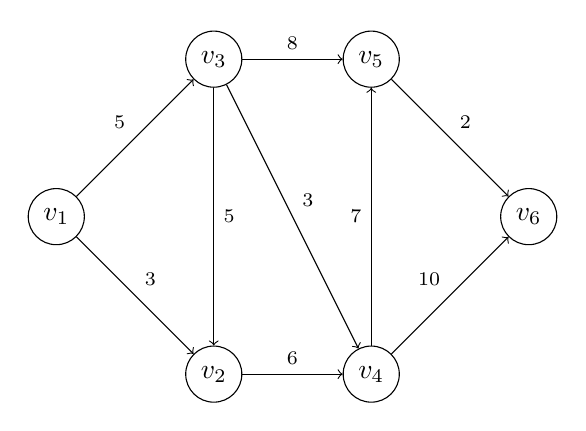
\begin{tikzpicture}[auto]
	% Knoten
		\node (1) at (0,0)  [circle,draw] {$v_1$};
		\node (3) at (2,2)  [circle,draw] {$v_3$};
		\node (2) at (2,-2) [circle,draw] {$v_2$};
		\node (5) at (4,2) [circle,draw] {$v_5$};
		\node (4) at (4,-2) [circle,draw] {$v_4$};
		\node (6) at (6,0) [circle,draw] {$v_6$};
	% Kanten
%		\path (1) -> node[weight] {$3$} (3)
		\draw[->] (1) edge node{\scriptsize 5} (3);
		\draw[->] (1) edge node{\scriptsize 3} (2);
		\draw[->] (3) edge node{\scriptsize 8} (5);
		\draw[->] (2) edge node{\scriptsize 6} (4);
		\draw[->] (3) edge node{\scriptsize 5} (2);
		\draw[->] (4) edge node{\scriptsize 10} (6);
		\draw[->] (3) edge node{\scriptsize 3} (4);
		\draw[->] (4) edge node{\scriptsize 7} (5);
		\draw[->] (5) edge node{\scriptsize 2} (6);
	\end{tikzpicture}
\end{document}